\chapter{Monte-Carlo Simulation} \label{sec::Samples}
Monte-Carlo (MC) simulation is a highly powerful toolkit providing theoretical prediction on event kinematics as well as the detector response, 
which is used extensively from studying signal/background separation, performance evaluation to background estimation. \\

This chapter discusses how the events are simulated, from some basics about the phenomenology in $pp$-collision, 
to the actual implementation in simulation where numerious approximations and simplifications are introduced. 
Referece \cite{ATLAS_generator} and \cite{SkandsQCD} are widely referred. 
Finally, the detailed configuration of each samples used in the analysis is overviewed.  \\


%%%
\section{Phenomenology of a $pp$-collision}
A typical $pp$-collision at the LHC energy can be understood and factorized by a number of different sub-processes:
\begin{description}

\item \textbf{Parton-level hard scattering} \mbox{} \\
The main process dominating the entire collision is the hard scattering where constituent partons in protons interact each other.  
The cross-section can be constructed by the matrix-element ($\mathcal{M}_{a,b\ra F}$; ME) from an initial state with the two partons ($a, b$) into a certain final state ($F$): 
\begin{align}
%\frac{d\sigma_{a,b \ra F}}{d\mathcal{O}} & = \int \frac{d\Phi}{d\bm{y}} \,\, |\mathcal{M}_{a,b \ra F}|^2 \,\, \delta \left( p^\mu_a + p^\mu_b - \sum_{i \in f} p^\mu_i   \right) 
\frac{d\hat{\sigma}_{a,b \ra F}}{d\bm{y}} & = \frac{1}{2 \hat{s}_{ab}} \frac{d\Phi}{d\bm{y}} \,\, |\mathcal{M}_{a,b \ra F}|^2  
\label{ppXsec}
\end{align}
where $\bm{y}$ represents momenta of final state particles; $d\Phi/d\bm{y}$ is the differential phase space; and the flux factor $1/2\hat{s}_{ab}$. 
The ME is the sum of transtion amplitude of all relevant processes with different intermediate states ($a,b \ra X \ra F$) characterized by different Feynman diagrams. \\


\item \textbf{Parton pick-up from a proton} \mbox{} \\
To translate the parton-level hard scattering into a $pp$-interaction,
one has to convolute with the parton distribution in a proton, for instance,
the parton-level cross-section Eq. \ref{ppXsec} is encapsulated by the parton distribution function (PDF):
\begin{align}
\frac{\mathrm{d}\sigma_{pp\ra F}}{\mathrm{d}\bm{y}} & = \sum_{i,j\in (q,\bar{q},g)} \int_0^1 \mathrm{d}x_a \int_0^1 \mathrm{d}x_b \,\, f_i (x_a) f_j (x_b) \,\, \frac{d\hat{\sigma}_{a,b \ra F}}{d\bm{y}}.
\label{ppXsecWithPDF}
\end{align}
$x_{a,b}$ denotes the momentum fraction of protons carried by the constituent parton $a,b$, and $f_i(x)$ is the PDF for parton flavor $i$ namely the probability density that one finds parton $i$ in the momentum fraction of $x$. $a$ and $b$ are finally added up with possible parton flavors, reflecting our ignorance on them.
Note that this convolution is not in terms of amplitude ($\mathcal{M}$) but rather a statistical addition,
ignoring the interference between the parton-level hard scattering and proton dynamics, which justified by the factorization theorem \cite{factTheoremQCD}. \\


\item \textbf{Additional parton radiation (ISR/FSR)} \mbox{} \\
Furthermore, additional jets often accompany from the splitting legs of initial and final state partons. 
They are referred as initial state radiation (ISR) or final state radiation (FSR). 
In principle, this effect should be counted as a part of parton-level hard scattering, 
however practically it is often useful to treat it as a separated auxiliary effect, as will shown later. 
\\


\item \textbf{Hadronization} \mbox{} \\
Resultant quarks and gluons in the final state are transformed into collections of fragmented hadrons  (``hadronization'').
This is particular the nature about the strong interaction known as ``confinement'' where the running coupling constant becomes stronger for longer distance scatterings and eventually diverges at the Laudau pole $Q^2\sim (200\mev)^2$. Naively this will lead to an infinite cross-section for processes with $Q^2\sim (200\mev)^2$, including quark and anti-quark pair productions out of the vacuum. 
\footnote{This is picture is incorrect giving the breakdown of perturbation, nevertheless enough to give an idea of the transition toward non-perturbative region.}
Those instantaneously generated partons are recombined eventually into hadrons with the singlet color state. This hadronization procedure can be understood using the the universal fragmentation function $D(z)$ in the same internal structure with PDF, representing the probability of finding a hadron with momentum fraction of $z$ with respect to that of seed parton. \\


\item \textbf{Underlying events} \mbox{} \\
Protons from which the hard scattering partons are kicked out are completely destroyed, no longer keeping the form as protons.
The remnants will experience their own hadronization, resulting in a splash of permeating hadronic background known as ``beam remnant''.
In addition, multiple parton-level scatterings (multiple parton interaction; MPI) occasionally take place within a single proton-proton interaction, where usually at least one of them ends up in a cheap QCD scattering leaving low-$\pt$ jets.
These sub-processes resulting in soft remnants as the background of the main hard scattering are inclusively referred to ``underlying events''. \\
\end{description}

Figure \ref{fig::Samples::ppCollisionScetch} is the schematic of the $pp$-collision with the sub-process.  \\

%The underlying event is a hadronic activity from a collision between partons of colliding hadrons
%not contribute to a hard process. The underlying event includes effects from the hadronisation of
%beam remnants and multiple 2 ! 2 parton interactions. 

%quarkとgluonはQCDのcharacteristical negative beta functionによってanti-screeningが起こって

%%%
%\fig[150]{Samples/ppCollisionScetch.pdf}
\figNoH[120]{Samples/ppCollisionScetch.pdf}
{Schematic of involved phenomenology in a $pp$-collision.}
{fig::Samples::ppCollisionScetch}
%%%


\section{Implementation of $pp$-collisions in Simulation}
Since it is practically non-calculable with the rigid formulation, 
what is implemented in the simulation is drastically simplified by employing numerical approach or approximation techniques. The detail for each sub-processes is described in this section. \\


\subsection{Parton Distribution Function}
Since the PDF is determined purely by non-perturbative dynamics, 
it is much easier to take the result of QCD measurement as the input rather than by first principle calculation.
A number of collaborations have performed 
a global fit on the experimental data of deep inelastic scatterings (DIS) or hadron-hadron collision mostly provided from HERA and Tevatron, with different parameterization and fitting scheme. 
Most frequently used sets in the LHC analyses are PDF4LHC \cite{PDF4LHC}, NNPDF \cite{NNPDF}, CT14 \cite{CT14}, MSTW \cite{MSTW}.
% and AZNLO \cite{AZNLO}. 
The uncertainties mainly results from instrumental uncertainties in the input data, uncertainties on the strong coupling constant and the functional form of parameterization.  \\
%Figure \ref{} shows ...


\subsection{Fixed-Order QCD Calculation}
The matrix-element in Eq. (\ref{ppXsec}) is computed based on the QCD and EW theory, with the truncated orders of perturbation series.
While the leading term in the perturbation (lowest order; ``LO'') dominates over the phase space, 
the inclusion of higher-order terms is significantly important for new physics searches.
This is because of the much smaller signal cross-section with respect to the SM backgrounds,
forcing one to explore the phase space where the bulk SM component is largely suppressed, 
in order to achieve a reasonable S/N. 
In such regions, typically the LO contribution is relatively more suppressed 
and the higher-order effects become addressing. \\

The calculation of higher-order terms are generally challenging giving the skyrocketing increased number of involved diagrams.
Currently, the cross-section calculation is available upto next-to-next-to-leading order (NNLO) for typical SM processes in LHC, and upto NLO level in event generation. Since the most phenomenologically important higher-order effect is the additional parton emission (ISR and FSR), 
there are also a class of generators dedicated for computing diagrams with the additional radiations (``multi-leg generators'') in the market, which can typically afford upto 4-9 additional partons at maximum, saving the computing resources by omitting the loop diagrams. \\


\subsection{Parton Showering}
On top of the straightforward QCD matrix-element calculation,
the parton shower (PS) approximation is further applied to supplement the description of the additional partons emission.
The concept is based on following two notions:

\begin{itemize}
\item Soft or collinear emission provide dominant contribution to the extra parton emission from a parton.
For instance, in $ee \ra q\bar{q} g$ as the minimal demonstration, the differential cross-section can be expressed:
\begin{align}
\frac{d\sigma_{q\bar{q}g}}{dx_1 dx_2} = \sigma_{q\bar{q}} \,\, \times \,\, \frac{\alpha_s}{2\pi} \frac{4}{3} \frac{x_q^2+x_{\bar{q}}^2}{(1-x_q)(1-x_{\bar{q}})}, \,\,\,\, x_i := 2E_i/\sqrt{s}
\end{align}
with $\sqrt{s}$ being the center-of-mass energy of the $ee$ system.
The appeared singularities correspond to the collinear emission of a gluon ($x_q \ra 1$ or $x_{\bar{q}} \ra 1$) or the soft gluon emission ($x_q \ra 1$ and $x_{\bar{q}} \ra 1$).
These collinear and soft singularities are universal to QCD, independent from type of processes. \\

\item In the soft/collinear regime, the cross-section with an additional parton radiation ($\mathrm{d}\sigma_{n+1}$) can be approximately factorized into the product of the original cross-section ($\mathrm{d}\sigma_{n}$) and the probability of the splitting $P_{i \ra j k}$:
\begin{align}
\mathrm{d}\sigma_{n+1} = \mathrm{d}\sigma_n \left[ \sum_{j,k} \,  \frac{\alpha_s}{2\pi} \, \frac{dq}{q} \, \frac{dz}{z} P_{i \ra j k} (z) \right],
\label{eq::PSSplit}
\end{align}
where the indices $i,j$ represent respectively the parent parton before and after the splitting, and $k$ the emitted parton. 
$z$ is the momentum fraction that the emitted parton $k$ carries from the parent $i$, and $q$ is the invariant mass (``virtuality'' when ignoring the quark mass) for the 4-momentum of the parton $i$. $P_{i \ra j k}$ is calculated as:
\begin{align}
P_{q \ra qg} & = \frac{4}{3} \frac{1+z^2}{1-z}, \nn \\
P_{q \ra gq} & = \frac{4}{3} \frac{1+(1-z)^2}{z}, \nn \\
P_{q \ra gg} & = 3 \frac{z^4+1+(1-z)^4}{z(1-z)}, \nn \\
P_{q \ra q\bar{q}} & = \frac{z^2+(1-z)^2}{2},
\label{eq::DEGLAP}
\end{align}
known as the Dokshitzer-Gribov-Lipatov-Altarelli-Parisi (DGLAP) evolution equations \cite{D_DEGLAP, L_DEGLAP, AP_DEGLAP}.
\end{itemize}

The parton shower technique is an emulation of the recursive parton splitting (``parton shower'') in a picture of stepwise evolution, in contrast to that in the matrix-element calcualtion where either initial and final state must be defined beforehand. 
The probability of emitting an extra parton at each step can be represented 
using Eq. (\ref{eq::PSSplit}) and Eq. (\ref{eq::DEGLAP})
analogous to the life-time of unstable particle decay :
\begin{align}
S_{i}(q_1, q_2) = 1 - \exp{ \left( -\sum_{j,k} \int_{q^2}^{q_{\mathrm{max}}^2} \frac{\mathrm{d}Q^2}{Q^2} \int_{z_{\min}}^{z_{\max}} \frac{\alpha_s}{2\pi} P_{i \ra j k}(\hat{z}) \mathrm{d}\hat{z}  \right)}
\label{eq::sudakov}
\end{align}
which is known as the Sudakov form factor \cite{Sudakov}.
$q_1$ ($q_2$) denotes the virtuality of parent parton before (after) the splitting.
%
FSRs are simulated by the evolution of final state parton legs with the splitting probability Eq. (\ref{eq::sudakov}), with an arbitrary initial virtuality. 
The evolution continues until the virtuality becomes the termination scale which is typically set to $\sim 1\gev$. ISRs are simulated in a similar manner but with a backward evolution with increasing virtuality. Generated sub-branches during the backward evolution are then evolved forward. The procedure is schematized as Figure \ref{fig::Samples::backwardEvolution}.

%%%
\fig[110]{Samples/backwardEvolution.pdf}
{Schematic of the backward evolution in the ISR simulation. 
The evolution starts with the parton entering the hard-scattering, with increasing the virtuality along the evolution. Partons split from the initial line are then evolved forward, in the same manner as the FSRs being generated.}
{fig::Samples::backwardEvolution}
%%%
Various implementation for the evolution exist, leading to a subtle difference in the final state kinematics. 
The impact are quoted as theoretical uncertainty in the analysis (see Sec. \ref{sec::Uncertainties::theoUnct}). \\

%It also particularly goes along with MC simulation since it does not require any try and acceptance so that no seed events will be discarded, enabling a highly computationally efficient generation. \\

Note that this shower evolution is fully pertubative though, it does include the contribution from arbitrarily higher order terms in the perturbation series (upto $n$-th order, where $n$ is number of parton splittings). Nevetheless, the imperfection of this appriximation is that it only accounts for the contribution from collinear and soft singularity. 
Therefore, a practical approach is commonly employed; generating as many ME-level partons as possible, and complementing the residual higher-order contributions by parton shwowering.
%This is the main motivation for multi-leg generators that provides hard ME-level additional partons to complement. 
One issue about this combined approach is the potential double-counting. The correction procedure commonly refers to ``matching'' or ``merging''. There are largely two types of correction; separating the region that each ME and PS is responsible for, in terms of phase space or scale. The most widely used algorithm is the Catani-Krauss-Kuhn-Webber (CKKW) \cite{CKKW_orig} algorithm or Michelangelo-L. Mangano algorithm (MLM) \cite{MLM}. ; Generating all jets by PS, and correct it by normalizing into the ME differential cross-section (ME correction).
\\

%\begin{itemize}
%\item 
% The CKKW ...
%MLM ..

%\item 
%This type of scheme is employed by \pythia and .
%\end{itemize}


\subsection{Hadronization}
%(jav need change)
A phenomenological approach is usually preferred for simulating hadronization. 
The most famous model is the Lund string model \cite{LundStringModel} where the interaction between the combinating partons is characterized by a gluonic string. 
For a quark-antiquark pair, as the partons move apart, the string is stretched leading to an increase in the potential energy. 
When the energy becomes of the order of hadron masses, it becomes energetically favorable for the string to break and create a new quark-antiquark pair. 
The two segments of string will be repeatedly pulled and break again, until all energy of initial quarks is converted into newly generated fragments. \\ \\ 
%Fragmentation function $D(z)$ is used to formulate the behavior ... \\


%\section{Underlying Events}
%A good understanding of underlying events is important from instrumental point of view, since it affects the calibrations of tracks %and objects. Several models and parameter tunes are available and are examined by data. Figure \ref{}.
% A14 ~\cite{ATL-PHYS-PUB-2014-021} for pythia 8
% P2012\cite{Skands:2010ak}  for  \pythia6.428~\cite{Sjostrand:2006za}


%\clearpage
\section{Setup of the Simulated Dataset}
%The generators used in the analysis are as below:
%\begin{itemize}
%\item \sherpa
%\item \powhegbox
%\item \mgmc
%\end{itemize}
\subsection{Event Generation} \label{sec:Samples::generators}
Events of the signal and background processes are generated using preferred generators and setups. 
Table \ref{tab::Samples::generators} summarizes the configurations for the simulated datasets.
Given that the analysis typically explores the phase space with many jets, 
physics processes with few hard tree-level jets (e.g. $\wzjets$, gluino production with compressed mass spectra etc.) need a dedicated modeling on ISRs and FSRs, 
for which the multi-leg generators (\sherpa, \madgraph) are preferred. 
For the other processes, events are simulated using the NLO generator $\powheg$. \\

\begin{table}[h]
  \begin{center}
    \caption{Setup of simulated SUSY signal and the Standard Model background samples. 
      $n_{\mathrm{ME}}^{\mathrm{a.p.}}$ denotes the number of simulated additional partons in the higher-order QCD processes.
      The column of ``PS/UE'' shows the programs in which parton showers and underlying events are generated.}
    \label{tab::Samples::generators}
    \begin{threeparttable}

      \begin{tabular}{c|cccc}
  \hline
  Physics process   &  Generator    &  $n_{\mathrm{ME}}^{\mathrm{a.p.}}$                      &  PDF set       & PS/UE  \\
  \hline
  \hline
  SUSY processes    &  \madgraph 2.3  $^\mathrm{a}$  &  2                 &  NNPDF2.3 LO                       & \pythia 8 $^\mathrm{d}$ \\
  $\wzjets$         &  \sherpa $^\mathrm{b}$         &  2(NLO)+2(LO)      &  NNPDF3.0 NNLO\cite{Ball:2014uwa}  & \sherpa         \\
  $\ttbar$          &  \powheg $^\mathrm{c}$         &  1                 &  CT10 \cite{Lai:2010vv}            & \pythia 6 $^\mathrm{d'}$    \\
  Single-top ($Wt$-ch.) &  \powheg v2                &  1                 &  CT10                              & \pythia 6      \\
  Single-top ($s$-ch.)  &  \powheg v2                &  1                 &  CT10                              & \pythia 6     \\
  Single-top ($t$-ch.)  &  \powheg v1 $^\mathrm{c'}$ &  1                 &  CT10f4                            & \pythia 6     \\
  Di-bosons              &  \sherpa                  &  1-2(NLO)+2-3(LO)  &  CT10                              & \sherpa        \\
  $\ttbar+W$   &  \madgraph 2.2  $^\mathrm{a'}$      &  2                 &  NNPDF2.3 LO                       & \pythia 8  \\
  $\ttbar+Z$   &  \madgraph 2.2                      &  1                 &  NNPDF2.3 LO                       & \pythia 8   \\
  $\ttbar+WW$   & \madgraph 2.2                      &  0                 &  NNPDF2.3 LO                       & \pythia 8  \\
  \hline
%
%%% footnotes
\end{tabular}
\begin{tablenotes}\footnotesize
\item[a] \MGMCatNLO 2.3.3 \cite{Alwall:2014hca}, NLO
\item[a'] \MGMCatNLO 2.2.3, LO
\item[b] \sherpatwo \cite{Gleisberg:2008ta}, NLO
\item[c] \textsc{powheg-box} v2 \cite{Alioli:2010xd}, NLO
\item[c'] \textsc{powheg-box} v1 \cite{Alioli:2010xd}, LO
\item[d] \pythiaeight  \cite{Sjostrand:2007gs}, LO, CKKW matching
\item[d'] \pythiasix \cite{Sjostrand:2006za}, LO, ME correction
\end{tablenotes}
\end{threeparttable}
\end{center}
\end{table}


% A14 ~\cite{ATL-PHYS-PUB-2014-021} for pythia 8
% P2012\cite{Skands:2010ak}  for  \pythia6.428~\cite{Sjostrand:2006za}
%
% pythia6 -> ME correction
% pythia8 -> CKKW-L
% Sherpa  -> CKKW
%

The simulated events are normalized by the total cross-sections that are separately calculated at a higher precision such as by including higher orders or the soft gluon resummation. 
Table \ref{tab::Samples::xsec} presents the summary of the total cross-sections and the configuration on which the they are calculated.

\tab{c|ccc}{
  \hline
  Physics process   &  Cross-section $[\mathrm{pb}]$   &  Order  & Authors \\
  \hline
  \hline
  SUSY processes    & See Figure \ref{fig::Samples::xsec_GG} &   NLO+NLL   & \cite{Beenakker:1996ch,Kulesza:2008jb,Kulesza:2009kq,Beenakker:2009ha,Beenakker:2011fu} \\
  $\wjets (\ra \ell\nu)$    & 20079                        &   NNLO      & \cite{Gavin:2010az}  \\
  $\zjets (\ra \ell\ell)$   & 1950                         &   NNLO      & \cite{Gavin:2010az}  \\
  $\ttbar$                  & 993.8                        &   NNLO+NNLL & \cite{topxs:2014} \\
  Single-top ($Wt$-channel) & 75.57                        &   NNLO+NNLL & \cite{wtxs:2014oha}  \\
  Single-top ($s$-channel)  & 10.32                        &   NLO       & \cite{Kant:2014oha} \\
  Single-top ($t$-channel)  & 216.95                       &   NLO       & \cite{Kant:2014oha} \\
%  Single-top ($Zt$-channel) & 0.24                         &   LO        & \mgmc 2.2.1   \\
  Di-bosons                  & 45.42                        &   NLO       & \cite{ATL-PHYS-PUB-2016-002}\\
  $\ttbar+W/Z/WW$           & 1.36                         &   NLO       & \cite{Lazopoulos:2008,Campbell:2012}\\
  \hline
}
{Cross-section used for the simulated processes. ``(N)NLL'' denotes the order upto which the soft gluon resummartion is taken into account.}
{tab::Samples::xsec}

%\clearpage
\noindent Further caveats particular to each process are noted in the appendix \ref{sec::Appendix::sample_detail}.
% ($W$/$Z$+jets)~\cite{ATL-PHYS-PUB-2016-003}

% -------------- xsec_GG
\begin{figure}[h]
  \begin{center}
    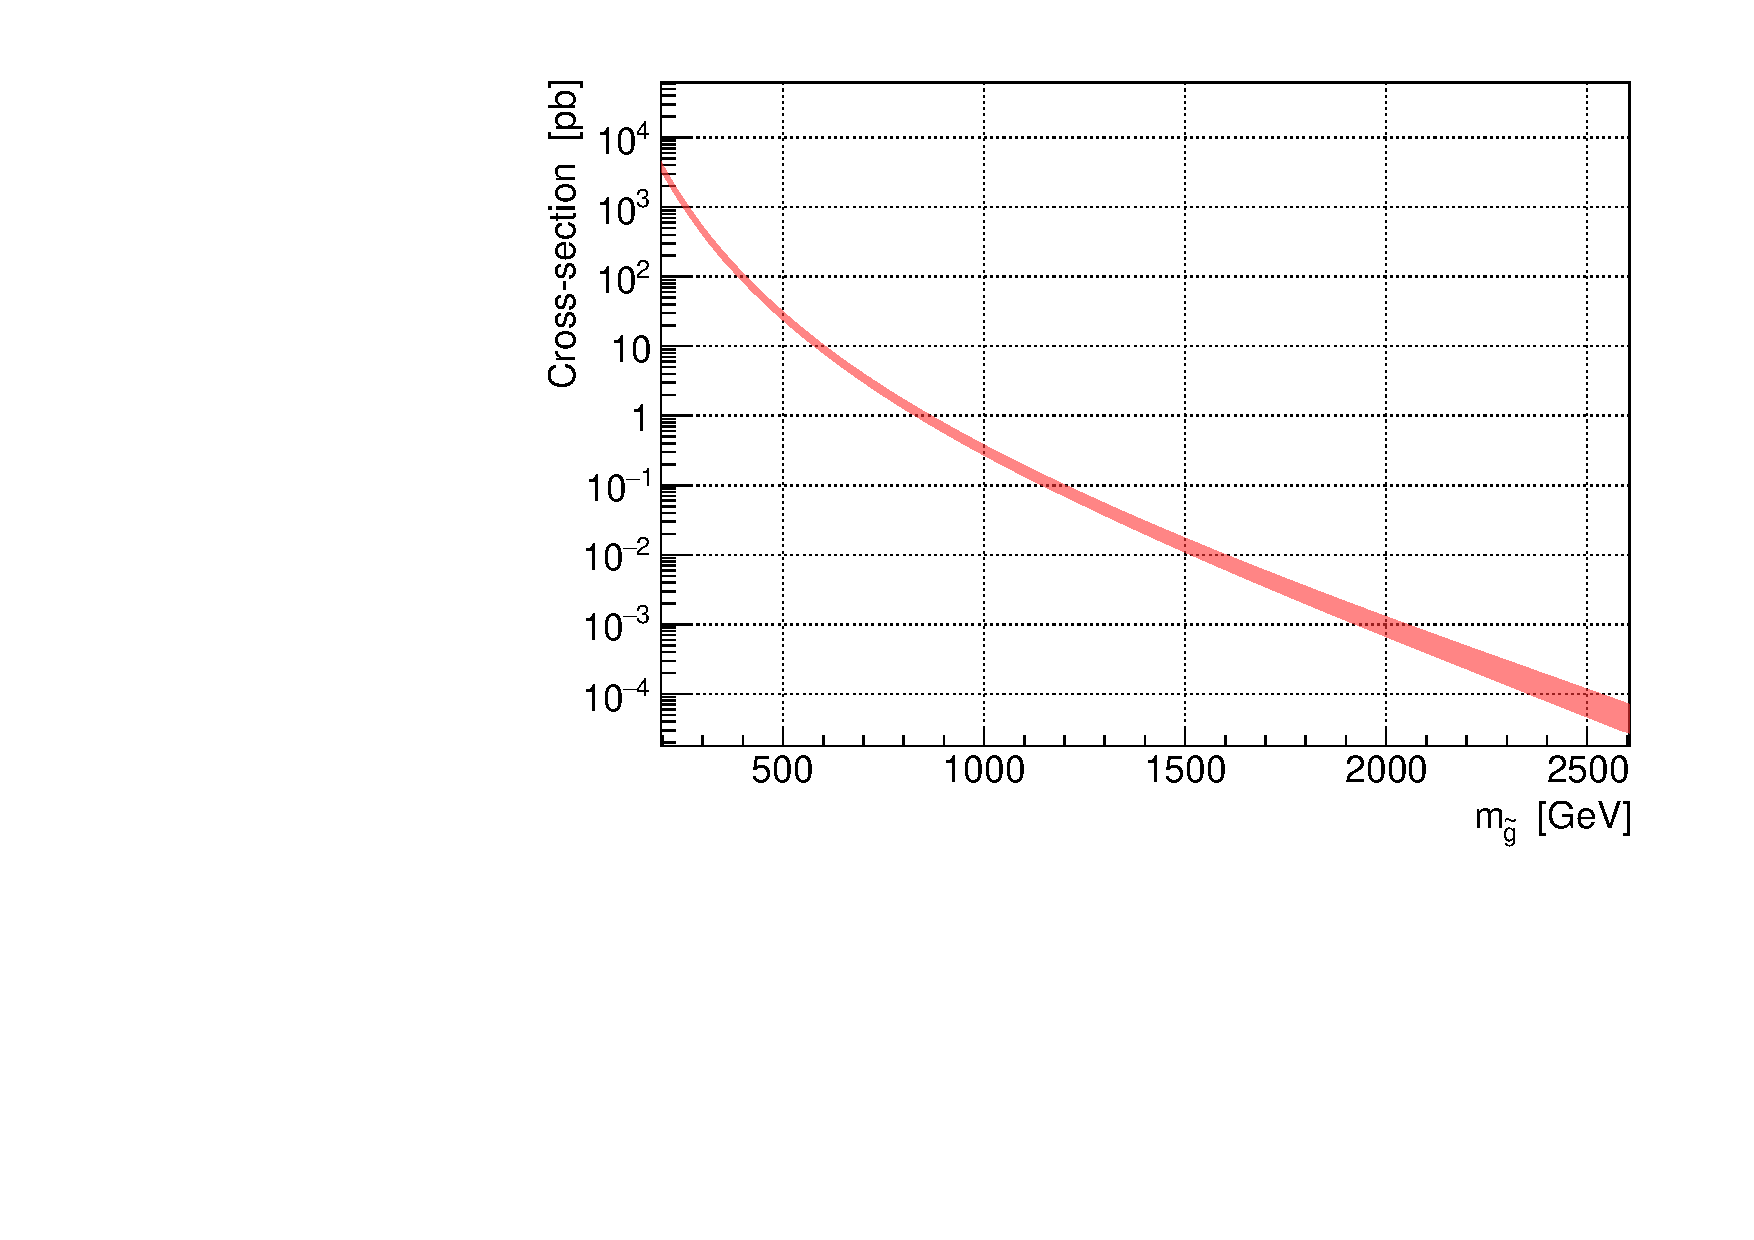
\includegraphics[width=120mm]{figures/Samples/xsec_GG/xsec_GG.pdf}
    \captionof{figure}{Cross-section of gluino pair production as function of gluino mass, at the NNLO+NNLL accuracy. The pink band corresponds to the calulation error.}
    \label{fig::Samples::xsec_GG}
  \end{center}
\end{figure}
%-------------------------------     



\subsection{Pileup simulation}
All simulated events are generated with a varying number of proton-proton collisions with soft QCD processes (minimum-bias interaction) overlaid on the hard-scattering event,
 to account for the pile-up in the same and the nearby crossing crossings.
The minimum-bias interactions are simulated with by \pythia8.186 using the A2 tune \cite{ATLAS:2012uec} and the MSTW2008LO PDF set~\cite{MSTW}. 
%Corrections are applied to the samples to account for differences between data and simulation for trigger, identification and reconstruction efficiencies. \\


\subsection{Detector Simulation and Emulation}
The detector response is simulated by a full ATLAS detector simulation model \cite{ATLASFullSimu:2010wqa} based on \textsc{Geant4}~\cite{Agostinelli:2002hh}, for the background samples. \\

The ATLAS fast simulation ~\cite{atlfast} is used as the economical alternative for part of the gluino signal processes (models marked as $\checkmark$ in Table \ref{tab::Introduction::modelsBV}-\ref{tab::Introduction::models3B} in Sec. \ref{sec::Introduction::targetModels}). 
This is based on a parametrization of the performance of the electromagnetic and hadronic calorimeters measured in the test-beam or on \textsc{Geant4}. 
The difference between the full simulation is found to be marginal after examining a number of reference signal points.
The subsequent procedures are identical to what is processed for the data sample. \\

For the signal models without $\checkmark$ in Table \ref{tab::Introduction::modelsBV}-\ref{tab::Introduction::models3B}, no detector simulation nor reconstruction is performed. Instead the effect is emulated by smearing the energy of truth-level particles and clustered jets, based on the resolution parameterized using the full simulated samples. The object identification is emulated by randomly accepting the candidates at the rate of the parameterized efficiency. The modeling is extensively tested by comparing the kinematic distributions with the fast simulated samples (see Sec. \ref{sec::App::valid_smear} in the appendix). The discrepancy is found sufficiently small, generally staying within $10\%\sim20\%$, which is acceptable given that the $15\%\sim35\%$ cross-section uncertainty on the gluino pair production. \\

% benchmark models
% non-benchmark models -> no detector simulation, use emulation


\section{Design of SUSY Signal Grid for Interpretation} 
Obtained exclusion limits are presented in a form of contours in a 2-dimensional plane, usually in terms of SUSY masses. This is done by generating a set of signal samples with various SUSY masses covering the whole plane with discrete steps, referred as a signal grid. The results of the hypothetical test on each point are eventually interpolated into a continuous profile. \\

For limits on the direct decay models, $\mG$ and $\mLSP$ are chosen as the $x$- and $y$-axis respectively (``$\dire$'' grid). The case with the 1-step decay models is a bit tricky, since they involve the third mass; the mass of the intermediate EW-gaugino ($m_{\chaone}$ or $m_{\neutwo}$). The full 3-dimensional presentation is not realistic from the computational cost of view. Therefore, a couple of sensible 2D-slices are made that sufficiently capture the essence of the 3D-grid. ``$\xhalf$'' is the grid with the intermediate EW-gaugino mass is set to the midmost between $\mG$ and $\mLSP$, while the splitting paramter $x$ is defined as the relative mass splitting:
\begin{align}
  \Delta m_{A,B} & := m_{A} - m_{B} \nn \\
  x & := \dmcn/\dmg, \,\,\,\,\,\,\, x \in [0,1]. \label{eq::def_x}
\end{align}
The ``\textttb{LSP60}'' grid is designed to complement the hole in high-$x$ or low-$x$, 
where the LSP mass is fixed to $60\gev$ while the masses of gluino and the intermediate EW-gaugino are set free. There are two additional DM-oriented grids (``\textttb{DM20}'' and ``\textttb{DM30}'') are defined in which the masses of the intermediate EW-gaugino and the LSP are compressed so that $\dmcn=20, \, 30\gev$ respectively, motivated by the dark matter relic constraint discussed in Sec. \ref{sec::Introduction::DMconstraint}. Note that the DM-oriented grids are not considered in models with $\neutwo$ decaying to higgs, since higgs is too far off-shell thus $\neutwo$ almost never decays via higgs in the situation. Table \ref{tab::Samples::signalGridDef} summarizies the designed signal grids in the analysis. 

\tabsmall{ c | c c c c}
%\tab{ c | c c c c}
{
\hline
Grid name   & x-axis   & y-axis         & Slicing                & Note\\
\hline
\hline
$\dire$       & $\mG$   & $\mLSP$         &  -                     & - \\
\hline
\hline
$\xhalf$      &  $\mG$  & $\mLSP$         &  $\dmg/2 = \dmcn$        & - \\
$\varx$       &  $\mG$  & $\dmcn / \dmg$  &  $\mLSP=60\gev$        & - \\
$\DMtw$, $\DMth$ &  $\mG$  & $\mLSP$         &  $\dmcn=20,30\gev$     & For models without \\
            &         &                 &                        & $h$-mediated $\tilde{\chi}_2^0$ decays. \\
\hline
}
{Types of the signal grids used for limit setting. $\dire$ is for the direct decay model, and the others are for the 1-step decay models. 
The latter is four-fold; $\xhalf$ where the intermediate EW gaugino mass is fixed to the midmost between $\mG$ and $\mLSP$; $\varx$ in which the LSP mass is fixed to 60$\gev$; $\DMtw$ and $\DMth$ are grids with $\dmcn=20,30\gev$ which are considered only in models without $\neutwo$ decay into higgs. }
{tab::Samples::signalGridDef}



